% Page settings
\documentclass[notitlepage,12pt]{article}
\usepackage{fancyvrb, verbatim, listings}                                  % Various for inserting/hosting code
\usepackage{setspace}                                                      % Space between lines (customisable)
\usepackage[margin=2.54cm]{geometry}                                       % Set margins (standard is 2.54cm)
\usepackage[UKenglish,cleanlook]{isodate}                                  % Set default date and date display
\usepackage{fancyhdr} \pagestyle{fancy}                                    % Line the top of the page
\usepackage[activate={true,nocompatibility},final,tracking=true,kerning=true,spacing=true,factor=1100,stretch=10,shrink=10]{microtype}
\microtypecontext{spacing=nonfrench}                                       % Change font and minor spacings to look nicer
\setlength{\parskip}{0.5\baselineskip}                                     % Set default paragraph behaviour: skip a line
%\setlength{\parindent}{0pt}                                                % Set default paragraph behaviour: no indent
%% Packages to use:
% Tables + figures
\usepackage{graphicx}                                                      % control over the import of graphics
\usepackage[table,dvipsnames]{xcolor}                                      % Define tables (with colour control)
\usepackage{float}                                                         % Control over graphics + tables float
\usepackage[justify]{ragged2e}                                             % control over text alignment
\usepackage{booktabs}                                                      % caption graphics + tables (with name in bold)
\usepackage[labelfont=bf]{caption} 
\usepackage{subcaption}
% caption graphics + tables (with name in bold)
\usepackage{tikz}                                                          % Draw graphs inline, guide: https://sites.google.com/site/kochiuyu/Tikz
\usetikzlibrary{shapes,decorations,arrows,calc,arrows.meta,fit,positioning}
\tikzset{
    -Latex,auto,node distance =1 cm and 1 cm,semithick,
    state/.style ={ellipse, draw, minimum width = 0.7 cm},
    point/.style = {circle, draw, inner sep=0.04cm,fill,node contents={}},
    bidirected/.style={Latex-Latex,dashed},
    el/.style = {inner sep=2pt, align=left, sloped}
}
\usepackage{pgfplots} \pgfplotsset{compat=1.16}                            % Automatic graphing, read https://www.overleaf.com/learn/latex/pgfplots_package for examples
\usepackage{subcaption}                                                    % Sub figures.
% Maths + numbers
\usepackage{mathtools}                                                     % Various maths functions
\usepackage{amssymb}                                                       % Various maths functions
\usepackage{amsmath}                                                       % Various maths functions
\usepackage{dsfont}                                                        % Various maths functions
\usepackage{centernot}                                                     % center \not usage
\usepackage{siunitx} \sisetup{round-mode=places, round-precision=3}        % Formalise use of units and numbers among text
\DeclareMathOperator{\eps}{\varepsilon}                                    % epsilon short hand shortcut
\DeclareMathOperator{\st}{\text{ s.t. }}                                   % "such that" short hand shortcut
\DeclareMathOperator{\then}{\text{ then }}                                 % "then" in equation shortcut
\DeclareMathOperator{\ifeq}{\text{ if }}                                   % "if" in equation shortcut
\DeclareMathOperator{\oreq}{\text{ or }}                                   % "or" in equation shortcut
\DeclareMathOperator{\andeq}{\text{ and }}                                 % "and" in equation shortcut
\DeclareMathOperator{\all}{,\; \forall}                                    % all (with spacing) in equation shortcut
\DeclareMathOperator{\N}{\mathbb{N}}                                       % N, natural number, shortcut
\DeclareMathOperator{\R}{\mathbb{R}}                                       % R, real number, shortcut
\DeclareMathOperator{\Ll}{\mathcal{L}}                                     % L, Lagrangian, shortcut
\renewcommand{\vec}[1]{\boldsymbol{\mathit{#1}}}                           % vector notation shortcut
\newcommand{\mat}[1]{\boldsymbol{\mathit{#1}}}                             % matrix notation shortcut
\DeclarePairedDelimiter\abs{\lvert}{\rvert}                                % absolute value notation shortcut
\DeclarePairedDelimiter\norm{\lVert}{\rVert}                               % norm notation shortcut
\newcommand{\Prob}[1]{\Pr\left( #1 \right)}                         % SHortcut for probability notation
\newcommand{\Probgiven}[2]{\Pr\left( #1 \, \middle\vert \, #2 \right)} % SHortcut for probability notation, given
\newcommand{\E}[2][]{\mathbb{E}_{#1} \left[ #2 \right]}                    % Expectation (with optional subscript) shortcut
\newcommand{\Egiven}[3][]{\mathbb{E}_{#1} \left[ #2 \, \middle\vert \, #3 \right]} % Expectation given (with optional subscript) shortcut
\newcommand{\Var}[2][]{\text{Var}_{#1} \left( #2 \right)}                  % Variation (with optional subscript) shortcut
\newcommand{\Cov}[1]{\text{Cov} \left( #1 \right)}                         % Covariance (with optional subscript) shortcut
\newcommand{\median}[1]{\text{median} \left( #1 \right)}                   % Median (with optional subscript) shortcut
\newcommand{\indicator}[1]{\mathds{1}\left\{ #1 \right\}}                  % SHortcut for indicator function
\newcommand{\diff}[2][]{\frac{d#1}{d#2}}                                   % SHortcut for differential fraction as a function
\newcommand{\partialdiff}[2][]{\frac{\partial#1}{\partial#2}}              % SHortcut for partial differential fraction as a function
\newcommand{\converge}[1]{\xrightarrow{ #1 \to\infty}}                     % SHortcut for convergence arrow
\renewcommand{\hat}[1]{\widehat{#1}}                                       % Default estimator notation is widehat
\renewcommand{\bar}[1]{\overline{#1}}                                      % Make over bar look nicer
\renewcommand{\tilde}[1]{\widetilde{#1}}                                   % Make over tilde look better
% Citations
\usepackage[longnamesfirst]{natbib}                                        % Citation package, see https://en.wikibooks.org/wiki/LaTeX/Bibliography_Management#Natbib
\usepackage[backref=page]{hyperref}                                        % Allow for links across the text, with colour options
\hypersetup{colorlinks=true, linkcolor=blue, citecolor=blue, filecolor=magenta, urlcolor=blue}
\def\equationautorefname~#1\null{Equation~(#1)\null}                       % Fix autoref for quations
% IMPORTANT: follow style guide here https://github.com/Wookai/paper-tips-and-tricks


%%%%%%%%%%%%%%%%%%%%%%%%%%%%%%%%%%%%%%%%
%% Title page
% Author
\author{Senan Hogan-Hennessy\thanks{
    Cornell University, Department of Economics.}
    \thanks{I thank Professor Evan Riehl for guidance on this project, Michael Lovenheim, Ronald Ehrenberg, Douglas Miller, and Francine Blau for various comments on the project's direction,
    as well as seminar participants at Cornell University (Spring 2022) for helpful
    discussion.
    This project's Github repository, with materials and (publicly available) data for replication, is available at 
    \url{https://github.com/shoganhennessy/finances-faculty-composition}.
    Any comments or suggestions may be sent to me at \href{mailto:seh325@cornell.edu}{\nolinkurl{seh325@cornell.edu}}, or raised as an issue on the Github project.}}
% Title
\title{Stagnating Public University Finances and Faculty Composition}
\date{\today}
\rhead{\today}
\lhead{Stagnating Public University Finances and Faculty Composition}
% Begin
\begin{document}
\clearpage \maketitle
\thispagestyle{empty}
% Abstract
\begin{abstract}
\noindent
\textbf{This needs re-doing}

When a worker's employer is exposed to demand shocks we may expect the resulting effect on the worker to depend on multiple economic factors, including size of the shock and the worker's outside options.
This paper studies the topic for a unique labour market: that of public university professors in the US.
State spending for public universities has secularly declined the last three decades, yet the isolated effects on professors are not yet clear.
Using an instrumental variables strategy to isolate shocks in public university revenues, I show that universities respond to negative revenue shocks by restricting employment among tenure-track and tenured professors -- possibly due to hiring and retirement channels, respectively.
Results using individual level data regarding every public university professor in Illinois are to follow.

\vspace{0.75cm}
\noindent\textbf{Keywords:} Public Sector Labor Markets, Higher Education, State and Local Budget and Expenditures

\vspace{0.5cm}
\noindent\textbf{JEL Codes:} J45, I23, H72
\end{abstract}
\newpage
\setcounter{page}{1}
%%%%%%%%%%%%%%%%%%%%%%%%%%%%%%%%%%%%%%%%%
%% Starting the paper
\newpage
\doublespacing


%%%%%%%%%%%%%%%%%%%%%%%%%%%%%%%%%%%%%%%%%
%% Plan
\subsection{Plan}
\begin{enumerate}
    \item Document empirical trend about number of professors per students, possibly diverging between private and public unis
    \item Document trend of falling revenues per student in the public sector -- while the private sector is fine
    \item Pull these facts together with shift-share IV approach to attribute the trend to falling state support for PUs.
    \item Document the effect on individuals in Illinois, including local projections for the dynamic effects.
    \item Theory discussion on the goals of a public university: public university charters require a minimum provision of teaching that make teaching a constraint, and other activities (including research).
    Implies exmploying fewer instructors per student, or substitution towards cheaper instructors who focus exclusively on teaching. 
\end{enumerate}


%%%%%%%%%%%%%%%%%%%%%%%%%%%%%%%%%%%%%%%%%
%% Introduction section
\section{Introduction}
\noindent
Public universities educate the majority of higher education students in the US, yet have experienced a secular decline in state funding (per student) the last few decades.
This decline has been shown to lead to worse education and later-life outcomes for students \citep{NBERw23736,NBERw27885}, yet it is not clear what institutional effects or mechanisms driving effects on students.
I show that four-year, degree-granting public universities (PUs) are exposed to tightening financial constraints thanks to falling state financial support (per student), and show this effects the composition of professors at PUs.
Falls in PU revenues, instrumented by state-level finance shocks, lead to a fall in the number of professors per student within a PU, driven by a fall in assistant or tenured professor counts.
US private universities are not exposed to similar financial constraints during this same time period, and do not exhibit any similar changes in the faculty composition, so that stagnating financial support for PUs have implications for the structure of higher education instruction and research in the US.

Universities in the US are widely considered the highest performing in the world,yet there are consequential differences between its universities that operate in the private sector and those established by state governments.
PUs are subject to numerous state-level administrative laws, and rely on their state governments for funding: an average PU received around \$11,600 per enrolled student in 1990, yet only \$8,300 per enrolled student in 2020.\footnote{
    2020 figures are relatively similar to those for year preceding, despite the Covid-19 pnademic and associated financial shocks, since 2020 refers to the academic year 2019-2020 and so the yearly budget was decided in 2019.
    This paper does not directly analyse budget shocks related to the Covid-19 pandemic, or any other events in 2020 and following.
}
This fall is driven by stagnating funding provided by state governments, while total enrollment among PUs rose by 46\% over the same time period.
At the same time, the number of professors per student at private universities stayed relatively stable at 0.045, yet fell from around 0.04 to around 0.35 professors per student at PUs, driven by a fall of over 20\% in the ratio of associate and full (i.e. tenured) professors per student at PUs.\footnote{
    \autoref{fig:fte-perprof} and \autoref{sec:trends} document these trends between private and public universities in full detail.
}

I use a variant of the \cite{NBERw23736,NBERw27885} shift-share instrument for PU revenues from shocks to state appropriations to identify the effect on the faculty composition.
State appropriations for public universities are plausibly endogenous to many outcomes: state governments decide on yearly budgets for their higher education sector, and this process can be influenced by local financial conditions, or even public (and political representatives') perceptions of the state's higher education system.
The shift-share instrument interacts reliance on state funding in a base period with the yearly total appropriations per student in the entire state;
the instrument for yearly state appropriations addresses the endogeneity concerns if state government funding decisions are not associated with any outcomes for any one university in the state \citep{NBERw27885}.
\autoref{sec:approp-shocks} provides further evidence in favour of the exogeneity assumption of the instrument.

Briefly describe results.

Then write about the Illinois data as individual-level data, and empirical approach when it is fully specified.

\cite{NBERw23736} first study the effect of (changes in) PUs' finances on student outcomes by isolating changes in PUs' expenditures on student instruction, addressing endogeneity of expenditures decisions by instrumenting expenditures by an instrument for state appropriations and tuition caps.
\cite{NBERw23736} find that increases in PU spending (via state appropriations) increases enrolment and degree completion among students, but corresponding changes in attendance price (via tuition caps/freezes) do not have an effect.
\cite{chakrabarti2018effect,NBERw27885} use the same instrument for PU revenues at the state level, combined with richer information on students' individual-level outcomes, to show that increases in state appropriations lead to lower time to completion and debt levels among students later in life.
\cite{bound2019public} use another variant of the same approach to show that state-level higher education spending cuts induced PUs to shift toward tuition as their primary source of revenue, and shift institutional resources towards students who pay higher tuition rates.
In a similar vein, \cite{bound2007cohort} document variation in per student state funding for higher education resulting from yearly changes in a state's student-age population; they find that lower per student funding lead to lower higher education completion rate among students.

University professors the core component of this country's educational and research/innovation university system, yet their composition within universities and its relationship with higher education finances has so far not been studied.
\cite{brown2014endowment} presents the closest example by studying how university endowments react to negative financial shocks, exhibiting an association between negative endowment shocks and a fall in tenure-system faculty employed at the university.
\cite{abe2015implications} present a model for university administrator decision-making, and posit that a large component of variation in faculty salaries arises from university politics, and not only economic factors such as outside.
\cite{johnson2009jep,NBERc13879} both empirically document allocation of faculty between research and instruction, and \cite{hemelt2021math} document differences in instructional cost (per student) between departments, primarily thanks to department differences in class size and faculty salaries.
\cite{turner2014impact} document how universities reacted to the Great Recession of 2008, a severe financial shock to state finances, including implementing hiring freezes.
Indeed, Cornell University\footnote{
    Cornell University is, indeed, only partially public, so that this information is not free information, and cannot be presented with aggregate or verified sources of public data on such salaries.
} implemented both hiring freezes and even a nominal salary reduction for professors, in anticipation of oncoming financial shock in early 2020.\footnote{
    The salary cut was not permanent, as the oncoming financial shock turned out to not be as serious as projected, and the salary cut was returned to professors in the year 2021.
}

The number of professors, in absolute terms as well as relative to number of students in the university, may be particularly important for quality of instruction and thus educational outcomes.
\cite{angrist1999using} first causally show that reducing class size induces an increase in test scores for school-age children, yet the magnitude of the effect is not as clear in the university setting.
\cite{bandiera2010heterogeneous} use a fixed effect model, combined with multiple individual observations in a long panel, to find that UK university students perform worse academically in particularly large classes, and the effect is particularly largest for students at the top of the academic distribution.
And for the composition of faculty teaching university classes, 
\cite{bettinger2010does,figlio2015tenure} find US students have better enrollment and learning outcomes from courses taught by contingent or adjunct (i.e. not tenured or on tenure-track) professors (relative to tenured or tenure-track).
While \cite{ehrenberg2005tenured} observe a negative association between utilisation of non-tenured instructors and student graduation rates.
My approach focuses on count of professors per student at universities, so does not directly observe individual class-sizes, yet presents this as a possible mechanism through which the negative effects on student outcomes that falls in PU finance \cite{NBERw23736,NBERw27885} document.

\textbf{Add in an intro conclusion paragraph.}
``Furthermore, because schools that serve students from lower-income backgrounds are most affected by state appropriations cuts, reductions in state support have helped exacerbate inequality and stratification of outcomes in the postsecondary sector.'' \citep{NBERw27885}.


%\begin{table}[H]
%    \centering
%    \caption{Table to Consider Impact of a Given Paper.}
%    \begin{tabular}{l | c c c c c}
%        & concepts & relationships & models & theories & use of methods \\
%        \midrule
%        
%        change:
%        & concepts & relationships & models & theories & use of methods \\
%        
%        challenge:
%        & concepts & relationships & models & theories & use of methods \\
%        
%        fundamentally alter:
%        & concepts & relationships & models & theories & use of methods \\
%    \end{tabular}
%\end{table}


%%%%%%%%%%%%%%%%%%%%%%%%%%%%%%%%%%%%%%%%%
%% Data section
\section{Data and Institutional Context}
\label{sec:data}

\subsection{Data Description}
The data used in this analysis come from two primary sources: \citet[IPEDS]{ipeds} regarding institutional information on finances and enrollment, and \citet[IBHED]{ibhed} for a panel of individual-level of every Professor employed by the Illinois PU system.

IPEDS is a survey of higher educational institutions in the US, and legally requires institutions to participate in order to receive Federal Title IV student aid.\footnote{
    This statement means that IPEDS does not necessarily cover the universe of US higher education institutions, yet thin practice every PU and not for-profit four-year institution is represented.
}
Data are consistent between the years 1990 and 2020,\footnote{
    The years 1987-1989 are represented in these data in an incompletion fashion, so I focus on the years 1990 onwards.
    Year refers to the calendar year of the spring term --- i.e. 1987 refers to the academic year that ran August 1986 to July 1987.
}
and provide information on the total revenues a university received from every source (including state governments), enrollment number, plus faculty count and total expenditures on salaries.\footnote{
    I combine the Urban Institute's 2018 compilation of IPEDS data for the years 1990-2017, and manually combine with raw NCES data regarding the year 2018-2020 for all relevant variables.
    Figures for enrollment, faculty counts and salaries come from the raw NCES version of IPEDS for all years to address inconsistencies in the Urban Institute's data formulation for these variables.
}
I restrict analysis to four-year institutions, as these institutions adhere to a standardised concept of faculty profile -- that is, tenure and title of appointment (lecturer, assistant professor, etc.) are relatively standardised in four-year, degree-granting institutions.
Additionally, for-profit institutions employ and enrol a negligible share of professors and students respectively, while students at two-year institutions by majority intend to eventually enroll at a four-year institution \citep{mountjoy2022}.\footnote{
    Furthermore, \cite{mountjoy2022} documents the effects of expanding two-year higher education access in the US separately for students who would have and those who would not have otherwise have attended college.
    The high rate of eventual enrollment at four-year institutions among two-year students explains the negative impact of increased access to two-year institutions on students who are diverted away from four-year institutions.
}

Importantly, IPEDS reports the count of professors employed by category, as well as total salary expenditures by category.
This gives a resulting panel data-set, where each row represents a university-year, and includes columns for university finances, plus total count and average salary\footnote{
    Real salary is computed by scaling nominal salary to 2021 dollars by the CPI-U.
} for professors by category (lecturer, assistant, tenured, total).
\autoref{tab:ipeds-summary} presents summary statistics for relevant variables in the panel of PU-years.

\begin{table}[h!]
    \onehalfspacing
    \centering
    \caption{IPEDS Summary Statistics, PUs Panel 1987--2020}
    \makebox[\textwidth][c]{
\begin{tabular}{@{\extracolsep{5pt}}lccc} 
\\[-1.8ex]\hline 
\hline \\[-1.8ex] 
Statistic & \multicolumn{1}{c}{Mean} & \multicolumn{1}{c}{St. Dev.} & \multicolumn{1}{c}{N} \\ 
\hline \\[-1.8ex] 
Enrolment & 11,511 & 10,821 & 18,504 \\ 
State appropriations (millions 2021 USD) & 99 & 125 & 18,504 \\ 
Total revenues (millions 2021 USD) & 425 & 793 & 18,504 \\ 
Non-institutional revenues (millions 2021 USD) & 202 & 265 & 18,504 \\ 
Lecturers count & 60 & 74 & 17,329 \\ 
Assistant professors count & 113 & 102 & 17,826 \\ 
Full professors count & 261 & 284 & 17,929 \\ 
All professors count & 429 & 437 & 18,504 \\ 
\hline \\[-1.8ex] 
\end{tabular} 
}
    \label{tab:ipeds-summary}
\end{table}

IPEDS provides information at the university level, yet lacks information on the distribution of salaries and professor count within a university.\footnote{
    IPEDS provides total paid to salary and total faculty employed per university-year, so that I can investigate average professor salary per university-year with IPEDS data.
    Unfortunately, it seems that this measure of professors' salaries is particularly crude in measuring on professors' salaries and other individual-outcomes; summary statistics on IPEDS data do not agree with trends in average professor salary over the sample time period \citep{aau2021survey}.
}
To investigate the distribution, I integregate individual-level data for every PU professor in the state of Illinois between the years 2010-2020.
IBHED host the information;
Public Act 96-0266 (effective 1 January 2010) requires that each PU report to the IBHE the base salary and benefits of the president and all administrators, faculty members, and instructors employed by the college or university.\footnote{
    The universities included are all campuses of the eight Illinois public universities: Chicago State University, Eastern Illinois University, Governors State University, Illinois State University, Northeastern Illinois University, Northern Illinois University, Southern Illinois University  (all five campuses), University of Illinois (all four campuses), Western Illinois University.
}
This publicly available data provides the basis to build a panel of Illinois PU professors 2010-2020; I define a professor as an individual observation by their first plus last name and university pairing, and link this database to IPEDS information on finances for their employing institution.
\begin{table}[h!]
    \onehalfspacing
    \centering
    \caption{IBHED Summary Statistics, Professor Panel 2011--2020.}
    \makebox[\textwidth][c]{
\begin{tabular}{@{\extracolsep{5pt}}lcccc} 
\\[-1.8ex]\hline 
\hline \\[-1.8ex] 
Statistic & \multicolumn{1}{c}{Mean} & \multicolumn{1}{c}{St. Dev.} & \multicolumn{1}{c}{Median} & \multicolumn{1}{c}{N} \\ 
\hline \\[-1.8ex] 
Lecturer, percent & 27 & 44 & 0 & 185,570 \\ 
Assistant professor, percent & 21 & 41 & 0 & 185,570 \\ 
Full professor, percent & 37 & 48 & 0 & 185,570 \\ 
Administrator professor, percent & 15 & 36 & 0 & 185,570 \\ 
Lecturer salary (2021 USD) & 31,650 & 25,825 & 27,474 & 49,637 \\ 
Assistant salary (2021 USD) & 77,075 & 38,078 & 73,387 & 39,051 \\ 
Full salary (2021 USD) & 109,535 & 48,949 & 100,044 & 68,243 \\ 
Administrator salary (2021 USD) & 119,462 & 61,377 & 107,824 & 28,639 \\ 
All salary (2021 USD) & 83,403 & 55,881 & 78,969 & 185,570 \\ 
Lecturer benefits (2021 USD) & 2,351 & 6,458 & 0 & 49,637 \\ 
Assistant benefits (2021 USD) & 2,964 & 7,092 & 0 & 39,051 \\ 
Full benefits (2021 USD) & 6,736 & 13,654 & 0 & 68,243 \\ 
Administrator benefits (2021 USD) & 3,607 & 15,976 & 0 & 28,639 \\ 
All benefits (2021 USD) & 4,286 & 11,547 & 0 & 185,570 \\ 
\hline \\[-1.8ex] 
\end{tabular} 
}
    \label{tab:illinois-summary}
\end{table}
The analysis sample focuses on the subset of professors with identified year of hiring between the years 2011 and 2020, representing 1,778 professors in 2011, and 9,099 in 2020.
\autoref{tab:illinois-summary} presents the summary statistics for this sample.\footnote{
    The full data IBHED contain 173,000 observations for every public university professor in Illinois 2010-2020, which representing 16,932 professors in the year 2010 and 15,352 in the year 2020.
    The reasons for restricting to the sample with identified year of hire in the range 2011-2020 is explained in \autoref{sec:iv-model-indiv}.
}

\subsection{Trends in Finances, Enrollment, and Faculty Composition}
\label{sec:trends}
A state government in the US plans an annual budget a couple of years ahead of the fiscal year, with the legislature approving a budget request put forth by the governor's office.\footnote{
    \cite{NBERw23736} present a full discussion of the state appropriation decision-making process, drawing on administrative records originally analysed by \cite{parmley2009state}.}
This process leads to yearly variation in state appropriations not seen in other revenues sources (such as federal government appropriations), since US states differ in their rate of (financial) support for higher education, and are subject to fiscal constraints.
US states governments, by majority, are legally obligated to run a balanced-budget, so that yearly variation in tax revenues (caused by changing economic conditions or otherwise) necessarily affect state expenditures.
State appropriations to higher education are a particularly attractive area of state spending to absorb such shocks to state finances \citep{delaney2011state}.\footnote{
    \cite{delaney2011state} fully describes the financial environment of state expenditures, and what makes spending on higher education an attractive area for state governments to expand funding during years of higher tax revenues, and retract funding in leaner years.
    An analysis of state expenditures for the years 1980-2004 (overlapping with the sample for this analysis) provides solid evidence for these trends.
}
Additionally, there is yearly state variation in the number of higher education students \citep{turner2014impact}, so that per-student state appropriations vary on multiple dimensions.

\autoref{fig:funding} exhibits the trends for the mean of US PUs between the years 1990-2020.
We see a rise in total revenues received by PUs (from all sources), and a notable increase in mean tuition revenues from \$48 million per year-university to \$150 million per year-university. 
Non-institutional revenues refer to revenues coming from external sources, not raised by internal university activities;\footnote{
    US universities raise revenues from many different internal activities, including sales of non-degree related educational courses to publishing deals.
    The non-institutional revenue measure is constructed to consider only revenues resulting from external decisions, including state, local, and federal appropriations and tuition revenues.
    Rates of tuition area considered external since most state governments play a large role in deciding tuition rices for PUs \citep{NBERw23736}.
}
non-institutional revenues rose over this time period almost exclusively thanks to the rise in tuition revenues.
At the same time, total state appropriations stagnated at around \$100 million per year-university for 1990-2008, fell slightly around 2008 and have not recovered.
While PUs experienced a financial stagnation, private universities were not exposed to the same constraints, receiving \$37,000 per student in 1990 and \$49,000 in 2020 with no corresponding decline in any specific component.

\begin{figure}[h!]
    \centering
    \caption{Mean Total Revenues among Public Universities, by Year.}
    \begin{subfigure}[b]{0.495\textwidth}
        \centering
        \caption{Total, millions \$ 2021 CPI-U.}
        \includegraphics[width=\textwidth]{figures/mean-funding-total.png}
        \label{fig:mean-funding-total}
    \end{subfigure}
    \begin{subfigure}[b]{0.495\textwidth}
        \centering
        \caption{Per Enrolled Student, \$ 2021 CPI-U.}
        \includegraphics[width=\textwidth]{figures/mean-funding-fte.png}
        \label{fig:mean-funding-fte}
    \end{subfigure}
    \label{fig:funding}
\end{figure}

At the same time, student enrollment at PUs rose precipitously.
6.2 million students were enrolled in PUs in 1990, and this number rose by 47\% to 9.1 million, with most of the increase occurring over the years 2000-2020.
\begin{figure}[h!]
    \centering
    \caption{Total Student Enrollment, by University Sector, and Year.}
    \begin{subfigure}[b]{0.495\textwidth}
        \centering
        \caption{Total.}
        \includegraphics[width=\textwidth]{figures/enrollment-total.png}
        \label{fig:enrollment-total}
    \end{subfigure}
    \begin{subfigure}[b]{0.495\textwidth}
        \centering
        \caption{Mean, University Level.}
        \includegraphics[width=\textwidth]{figures/enrollment-mean.png}
        \label{fig:enrollment-mean}
    \end{subfigure}
    \label{fig:enrollment}
\end{figure}

\autoref{fig:enrollment} shows that total enrollment at private universities has also risen over the same time period, but not as drastic in either relative or absolute terms; the mean public university also grew over this time period, from 9,800 students in 1990 to 11,800 in 2020.
This means that per student mean revenues per student (seen in \autoref{fig:mean-funding-fte}) have stagnated across all measures, and particularly fallen from \$11,000 per student in 1990 to less than \$8,000 per student in 2020.
\begin{figure}[!h]
    \centering
    \caption{Total Professor Count per Student, by University Sector, Professor Appointment, and Year.}
    \begin{subfigure}[b]{0.495\textwidth}
        \centering
        \caption{Lecturer}
        \includegraphics[width=\textwidth]{figures/lecturer-fte-perprof.png}
        \label{fig:lecturer-fte-perprof}
    \end{subfigure}
    \begin{subfigure}[b]{0.495\textwidth}
        \centering
        \caption{Assistant.}
        \includegraphics[width=\textwidth]{figures/assistant-fte-perprof.png}
        \label{fig:assistant-fte-perprof}
    \end{subfigure}
    \begin{subfigure}[b]{0.495\textwidth}
        \centering
        \caption{Full.}
        \includegraphics[width=\textwidth]{figures/full-fte-perprof.png}
        \label{fig:full-fte-perprof}
    \end{subfigure}
    \begin{subfigure}[b]{0.495\textwidth}
        \centering
        \caption{All.}
        \includegraphics[width=\textwidth]{figures/all-fte-perprof.png}
        \label{fig:all-fte-perprof}
    \end{subfigure}
    \label{fig:fte-perprof}
\end{figure}

\autoref{fig:fte-perprof} documents the divergence in faculty composition (per student) between the average private and public university 1990-2020.
Private universities start with  a higher baseline of around 4.5 professors per 100 students, and exhibits yearly variation of less than 0.5 professor per 100 students over the thirty years.
PUs start with 3.9 professors per student, and this number falls to 3.5 primarily in the 2008-2011 time period.
We see a similar difference in baseline, and fall for the years 2008-2011 for assistant professors.
Private and public universities have similar numbers of associated and full professors before thea year 2000, yet this number has fallen by over 20\% in the next 20 years only for PUs: in 2020 the mean PU has 6 fewer full professors per tudent than the mean private university.
At the same time period, we see the rise in use of non-tenure track instructor positions (referred to as lecturers from here on), who were employed at similar rates in both sectors in 1990 yet have been utilised by PUs at a higher rate since.


%%%%%%%%%%%%%%%%%%%%%%%%%%%%%%%%%%%%%%%%%
%% Empirical section
\section{Empirical Framework}
\label{sec:empirics}

A professor is employed by a university, so it stands to reason that when PUs experience a secular fall in revenue --- analogous to a demand shock in the private sector --- that their human resources decisions will be affected.
Universities have been shown to freeze faculty hiring and general faculty salaries in response to financial shocks, such as the Great Recession \citep{turner2014impact}.

Na\"ively we can analyse the relationship between professor-outcomes $Y_{i,t}$ at university $i$ in year $t$ as a result of university revenues per student $X_{i,t}$.
Professor outcomes include count of professors per student, and average salary, within each university-year.
This model gives $\beta$ the association with these outcomes and university revenues per student,\footnote{
    Note that dividing by student count also implicitly controls for the size of the university, so that this model accounts for yearly variation in professor count and university revenues arising from growth in a university.
}
including fixed effects to control for effects specific to the university and year.
Log$(.)$ transforming the variables improves the interpretability of $\beta$ as an elasticity for professor count per student with respect to institution revenues.
\begin{equation}
    \label{eqn:naivereg}
    Y_{i,t} = \alpha_i + \gamma_t + \beta X_{i,t} + \epsilon_{i,t}
\end{equation}

And yet a university's finances are not exogenous to decisions made by the university administrator (such as hiring), state outcomes or enrollment.
Instead, the state government and university administration undertake a complex process of alloting resources across multiple different priorities, including instruction, research, or between departments.
Importantly for this analysis, revenues received from a  PU's state government provide opportunity to address this endogeneity.


\subsection{State Appropriation Shocks}
\label{sec:approp-shocks}

\cite{NBERw23736,chakrabarti2018effect,NBERw27885} address endogeneity in PU finances by exploiting a shift-share instrument for changes in state-level funding interacted with university reliance on state funding in a base period.
The system exploits the fact that institutions who rely on state appropriations more will be affected by later shocks to state appropriations.
We start with the shift-share instrument.
\begin{align}
    \label{eqn:public-instrument}
    Z_{i,t} &\coloneqq \log \left[
    \left( \frac{\text{Total State Funding}_{s(i),t}}{\text{Student Population}_{s(i),t}} \right)
    \sum_{\tau = 0}^{3} \frac 14
    \left( \frac{\text{State Funding}_{i,1990 + \tau}}{\text{Total Revenues}_{i,1990 + \tau}} \right) \right]
\end{align}

$Z_{i,t}$ is the instrument for (log) state appropriations for institution $i$ in year $t$, interacting the average funding for university $i$ in state $s(i)$ with reliance on state funding relative to total revenues, averaged across the base years 1990--1993.\footnote{
    1990--1993 are defined as data for PU finance data are most comparable (i.e. without many missing values) beginning in 1990.
    \cite{NBERw23736} use the single year 1990 as the base year, though I use the four years to ameliorate missing values in the single year of 1990.
    Results are similar in either specification.
}
\cite{NBERw27885} notes the tendency for PUs to respond to state funding cuts by increasing reliance on tuition, where \cite{NBERw23736} specifically instruments for tuition revenues with collected information on legislative tuition price controls.
As such, it is important in my set-up to explicitly control for tuition revenues in the first-stage.

The first-stage is then as follows, where $W_{i,t}$ represents (log) tuition revenues, including institution and year fixed effects.
\begin{equation}
    \label{eqn:firststage}
    X_{i,t} = \eta_i + \zeta_t + \delta Z_{i,t} + \kappa W_{i,t} + \epsilon_{i,t}
\end{equation}
We note the conditions for exogeneity in the instrument (following the discussion presented by \citealt{NBERw27885}).
The instrument is exogenous if state policy decisions for funding of, or tuition charges by PUs, are uncorrelated with unobserved changes in the expenditures of any specific college or university in the state.
This assumption is plausible given that the majority of states have multiple (i.e. more than five) public universities, without any single university campus receiving the majority of state funding within any single state.
Secondly, addressing endogeneity in university revenues by the shift-share identification strategy requires exogeneity in either the base-line share or shift component of the instrument.
In this case, we satisfy the second: universities' institutional-level decisions are not correlated with contemporaneous or upcoming shocks to state appropriations.\footnote{
    It would be plausible to consider the case that universities make institutional-level decisions in a consistently different manner to those 
    with differing reliance on state appropriations in 1990, so that exogeneity by the base-line share is not plausible here.
}

\autoref{tab:firststage-reg} presents results of the first-stage regression, separately with and without the tuition control and fixed effects, at the institution level (i.e. using IPEDS data).\footnote{
    Representations for frequentist significance levels (i.e. 10, 5, 1\% etc.) are omitted here, and in all following tables.
}
\begin{table}[!h]
    \onehalfspacing
    \centering
    \caption{First Stage Estimates, for Total University Revenues by Shocks}
    \makebox[\textwidth][c]{
\begin{tabular}{@{\extracolsep{5pt}}lcccc} 
\\[-1.8ex]\hline 
\hline \\[-1.8ex] 
 & \multicolumn{4}{c}{Dependent Variable: State Funding} \\ 
\cline{2-5} 
\\[-1.8ex] & (1) & (2) & (3) & (4)\\ 
\hline \\[-1.8ex] 
 Funding Shift-share& $-$0.977 & $-$0.302 & $-$0.986 & $-$0.573 \\ 
  & (0.066) & (0.093) & (0.062) & (0.067) \\ 
  Tuition Revenue &  &  & 0.058 & 0.535 \\ 
  &  &  & (0.059) & (0.065) \\ 
  Constant &  & 6.419 &  & $-$0.484 \\ 
  &  & (0.769) &  & (0.844) \\ 
 \hline \\[-1.8ex] 
Uni. + Year fixed effects? & Yes & No & Yes & No \\ 
F stat. & 249.662 & 74.022 & 218.171 & 10.558 \\ 
Observations & 17,012 & 17,012 & 17,012 & 17,012 \\ 
R$^{2}$ & 0.790 & 0.047 & 0.790 & 0.180 \\ 
\hline 
\hline \\[-1.8ex] 
\end{tabular} 
}
    \label{tab:firststage-reg}
    \begin{flushleft}
        \footnotesize
        \textbf{Note}: Standard errors are clustered at the state-year level.
    \end{flushleft}
\end{table}
We note columns (1) and (2) estimate that a shock to state appropriations per student in the state of 10\% is associated with around 2.5\% change in non-institutional revenues per student at the university; the instrument is strong, and we note similarity in estimates with and without inclusion of fixed effects.
Columns (3) and (4) exclude the tuition revenue control (explained above) to exhibit bias in the first-stage if it is not controlled for.
Column (3) shows similar estimates to columns (1), (2) thanks to inclusion of fixed effects, so that the fixed effects was effective in soaking variation in per-student tuition revenues at the institution-year level.
Column (4) exhibits the worst case, and extreme bias in the appropriation shock first-stage without the tuition control.
Column (1) represents the estimates for \autoref{eqn:firststage} with fixed effects, and is the preferred form that I proceed with in the following.

\autoref{fig:firststage-lp} presents local projection estimates for the staying-power of the state appropriation shock to university revenues.
We see the time 0 estimate coincides with that of Column (1) in \autoref{tab:firststage-reg}, the contemporaneous effect of the shock revenues.
We see a decaying, yet real and positive, effect of the shock on revenues for the next 5 years, illustrating the staying power of the effect.

\begin{figure}[h!]
    \centering
    \caption{Local Projection Estimates for First-Stage \autoref{eqn:firststage}.}
    \includegraphics[width=0.6\textwidth]{figures/firststage-lp.png}
    \label{fig:firststage-lp}
\end{figure}

These results, together with the case for exogeneity, show the appropriations shock instrument strongly predicts university revenues in the first-stage estimation.


\subsection{Instrumental Variables Model, University-Level}
\label{sec:iv-model-uni}

The primary empirical model combines the instrumental variable for stata appropriation shocks with the empirical model for the effects of university revenues at the university-level -- i.e. parameter $\beta$ in the following.\footnote{
    It is important to note the treatment effect isolated here; the instrumental variables approach identifies the local average treatment effects (LATE) specific to the instrument.
    So we interpret this treatment effect as the PU's response in employment count and average salaries to revenue changes, changes specific to state appropriation shocks, among the complier group --- i.e. universities with any exposure to shocks, assuming no universities increase employment or salaries in response to revenue shocks.
    \cite{mogstad2021causal} provide a full discussion of the LATE with multiple instruments and thus multiple monotonicity conditions.
}
\begin{eqnarray}
    \label{eqn:secondstage1}
    X_{i,t} &=& \eta_i + \zeta_t + \delta Z_{i,t} + \kappa W_{i,t} + \epsilon_{i,t} \\
    \label{eqn:secondstage2}
    Y_{i,t} &=& \alpha_i + \gamma_t + \beta \widehat X_{i,t} + \lambda W_{i,t} + \varepsilon_{i,t}
\end{eqnarray}
I estimate the system by two stage least squares, including institution and year fixed effects, and investigate outcomes at the university-level to analyse effects on the university as a result of changes in revenues.
Additionally, I estimate the model via local projections \citep{jorda2005,miller2022} to investigate whether the effects of revenues on faculty composition linger for multiple years after the original appropriation shock.
Regarding outcomes, I focus on the composition of the professors employed at the university by analysing (log) count per student, and average salaries paid to, professors employed by the university.

\begin{figure}[H]
    \centering
    \caption{Instrument Variables Model for University Finances and Faculty Composition.}
    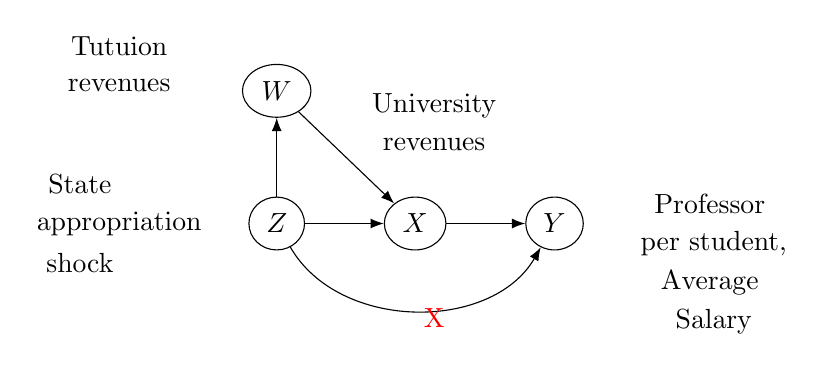
\begin{tikzpicture}
        \node[state] (instrument) at (0,0) {$Z$};
        \node at (-2.5,0.5){State};
        \node at (-2.0,0){appropriation};
        \node at (-2.5,-0.5){shock};
        \node[state] (confounder) [above=of instrument] {$W$};
        \node at (-2,2.25) {Tutuion};
        \node at (-2,1.75) {revenues};
        \node[state] (endogenous) [right=of instrument] {$X$};
        \node at (2,1.5) {University};
        \node at (2,1) {revenues};
        \node[state] (outcome) [right=of endogenous] {$Y$};
        \node at (5.5,0.25) {Professor};
        \node at (5.55,-0.25) {per student,};
        \node at (5.5,-0.75) {Average};
        \node at (5.55,-1.25) {Salary};
        % Relevance condition
        \path (instrument) edge (endogenous);
        \path (endogenous) edge (outcome);
        % Confounding relationship
        \path (instrument) edge (confounder);
        \path (confounder) edge (endogenous);
        % Exclusion Restriction
        \path (instrument) edge[bend right=60] (outcome);
        \node[color=red] at (2,-1.2) {X};
    \end{tikzpicture}
    \label{fig:SCM-ivmodel}
\end{figure}

\autoref{fig:SCM-ivmodel} presents the system in graphical format, where tuition revenues $W$ are considered a confounder in the causal effect of state appropriation shocks on total revenues.


\subsection{Instrumental Variables Model, Individual Professor-Level}
\label{sec:iv-model-indiv}

This analysis additionally utilises data regarding individual professors in the Illinois university system, to investigate the effects of changes in university revenues on the individual professors at the universities.
Yet, redefining the level of outcome requires adjustment to the empirical approach to leverage variation in university finances in the years following an individual joins the university.\footnote{
    This formulation follows that presented by \cite{NBERw27885}, where individual student outcomes are analysed via variation in state appropriations after their freshman-year.
    This constrasts with \autoref{sec:iv-model-uni} and \cite{NBERw23736}, where the unit of analysis is the university-year.
}

\autoref{eqn:public-instrument} defines a rolling-share variant of the instrument, $\tilde Z_{j,t}$, where the university's share exposure to state appropriations is based the year a professor joins the university --- and not the base period 1990--1993.
$j$ indexes each professor in year $t$, $\tau(j)$ for the year the professor first joins their Illinois PU.\footnote{
    Identifying $\tau(j)$ is possible for $j$ by restricting to all professors who are hired in the time period 2011-2020 (i.e. in the years after the first in the panel).
    Professors who were hired in the year 2010 are impossible to distinguish from those in year preceding, and so are not considered.
}
\begin{align}
    \label{eqn:rolling-instrument}
    \tilde Z_{j,t} &\coloneqq \log \left[
    \left( \frac{\text{Total State Funding}_{s(j),t}}{\text{Student Population}_{s(j),t}} \right)
    \left( \frac{\text{State Funding}_{\tau(j)}}{\text{Total Revenues}_{i,\tau(j)}} \right) \right]
\end{align}

This approach leverages an insight, made available by level of the data: that an individual professor is affected by changes in university revenues after they have joined the university.\footnote{
    Notice that \autoref{sec:iv-model-uni} considers a the number of professors employed by the university.
    So that whether a professor becomes employed at the university is likely affected by the university revenues.
    The formulation in this section does not consider that outcome, instead taking as given that the professor is employed at the university, and then projecting the effect on the individual given they are employed here.
}
Exogeneity and relevance of the rolling-share instrument, $\tilde Z_{j,t}$, follows the same reasoning as that for the base-share instrument, $Z_{i,t}$, discussed in \autoref{sec:approp-shocks}.
We satisfy the assumptions by noting that none of the Illinois public campuses take the majority of state appropriations, and that the instrument identification strategy relies on exogeneity in changes in state appropriations to individual professor-outcomes, following the year they joined the university.\footnote{
    Additionally, within-institution changes resulting from share reliance on state funding may be correlated with unobserved changes in the outcomes, so that \cite{NBERw27885} note the importance of controlling for the base share and state student population.
    My formulation implicits controls for these factors via the fixed effects; results are relatively similar while including these controls without including fixed effects.
}
\autoref{tab:firststage-illinois} presents results of the first stage estimation, showing that the instrument is strong (after conditioning on tuition revenues) in the same way as that for the university-level outcomes (\autoref{tab:firststage-reg}), with very similar estimates for the association between appropriation shocks and non-institutional revenues.

The full model is defined as follows where $i(j)$ refers to the institution that professor $j$ is employed at, and $Y_{j,t}$ refers to individual-level outcomes total salary, rate of promotion, and propensity to leave the Illinois PU system.
The system includes a fixed effect for the institution and first year of employment.\footnote{
    The instrument varies by institution, based in the year of first employment so that these are the corresponding fixed effects and levels of clustered standard errors.
}
\begin{eqnarray}
    \label{eqn:secondstage1_indiv}
    X_{i(j),t} &=& \theta_{i(j)} + \phi_{\tau(j)} + \delta \tilde Z_{i(j),t} + \kappa W_{i(j),t} + \epsilon_{i(j),t} \\
    \label{eqn:secondstage2_indiv}
    Y_{j,t} &=& \mu_{i(j)} + \nu_{\tau(j)} + \beta \widehat X_{i(j),t} + \lambda W_{i(j),t} + \varepsilon_{i(j),t}
\end{eqnarray}
We then interpret parameter $\beta$ in this formulation as the effect of changes in university revenues, via state appropriation shocks, on an individual professor.


%%%%%%%%%%%%%%%%%%%%%%%%%%%%%%%%%%%%%%%%%
%% Results section
\section{Results}
\label{sec:results}

\subsection{University-Level}

\autoref{tab:facultycount-shock-reg} presents OLS and IV estimates, where the outcome is (log) count of professors employed at the university, separated by group and combined (columns 7, 8).
Within each group we see a positive correlation between university revenues and professor count per student (the OLS columns), where an increase in university total revenues by 10\% is associated with an increase in professor employment count between 3.5-4.5\%.
Lecturers per student is not shown to be correlated with total univesity revenues.
The 2SLS columns show results after identifying university revenues with the appropriation shock.
All professor count per student increases by 3\% in response to a 10\% rise in total revenues, mediated by revenue shocks.
The effect is driven by increases in the count of assistant and full professors (i.e. tenure-track and tenured) per student, where assistant professor count per student increase by 6.7\%, and full professor 5\%.
The count of lecturers per student decreases by 12\% in response to a (positive) 10\% shock in university revenues.

\begin{table}[!h]
    \onehalfspacing
    \centering
    \caption{OLS and 2SLS Estimates for University Faculty Composition.}
    \makebox[\textwidth][c]{
\begin{tabular}{@{\extracolsep{5pt}}lcccccccc} 
\\[-1.8ex]\hline 
\hline \\[-1.8ex] 
 & \multicolumn{8}{c}{Dependent Variable: Employment Count by Professor Group} \\ 
\cline{2-9} 
\\[-1.8ex] & \multicolumn{2}{c}{Lecturer} & \multicolumn{2}{c}{Assistant} & \multicolumn{2}{c}{Full} & \multicolumn{2}{c}{All} \\ 
 & OLS & 2SLS & OLS & 2SLS & OLS & 2SLS & OLS & 2SLS \\ 
\\[-1.8ex] & (1) & (2) & (3) & (4) & (5) & (6) & (7) & (8)\\ 
\hline \\[-1.8ex] 
 Non-inst. Revenues & $-$0.059 & $-$1.426 & 0.348 & 0.659 & 0.453 & 0.530 & 0.360 & 0.310 \\ 
  & (0.162) & (0.590) & (0.126) & (0.207) & (0.154) & (0.134) & (0.144) & (0.100) \\ 
  Tuition Revenue & 0.432 & 0.951 & 0.091 & $-$0.028 & $-$0.060 & $-$0.090 & 0.040 & 0.059 \\ 
  & (0.103) & (0.234) & (0.098) & (0.101) & (0.080) & (0.065) & (0.061) & (0.053) \\ 
 \hline \\[-1.8ex] 
Observations & 17,329 & 17,329 & 17,826 & 17,826 & 17,929 & 17,929 & 18,504 & 18,504 \\ 
R$^{2}$ & 0.673 & 0.631 & 0.720 & 0.712 & 0.794 & 0.793 & 0.827 & 0.827 \\ 
\hline 
\hline \\[-1.8ex] 
\end{tabular} 
}
    \begin{flushleft}
        \footnotesize
        \textbf{Note}: Standard errors are clustered at the state-year level.
    \end{flushleft}
    \label{tab:facultycount-shock-reg}
\end{table}

DISCUSS WHAT THOSE POINT ESTIMATES MEAN, DISCUSSING THE POSSIBILITY THAT LECTURERS ARE INFERIOR GOODS, TENURE TRACK NORMAL GOODS.


This finding is particularly in line with the \cite{turner2014impact} observation regarding hiring freezes particularly for tenure-track hirings, and \cite{brown2014endowment} from shocks to endowments.
Similarly, the effect is exhibited on order of 2.6\% among full professors (those holding tenure), likely through the channel of retirements or replacement hirings (since tenured professors cannot be forcibly fired/not renewed without cause).

Write something about the level of tenure, and that data are available for a subset of years, and shown in Appendix \autoref{tab:tenurecount-shock-reg-fte}.

\autoref{fig:all-count-lp} shows local projection estimates, staying power of the effect on prof count.

\begin{figure}[h!]
    \centering
    \caption{Local Projection Estimates for Professor Count per Student.}
    \includegraphics[width=0.6\textwidth]{figures/all-count-lp.png}
    \label{fig:all-count-lp}
\end{figure}

WRITE HERE ABOUT STAYING POWER.


\subsection{Individual Professor Outcomes}

Estimates for the model where units of analysis are individual professors at Illinois PUs follow.

\begin{table}[!h]
    \onehalfspacing
    \centering
    \caption{2SLS Estimates for Faculty Salaries at Illinois Universities.}
    \makebox[\textwidth][c]{
\begin{tabular}{@{\extracolsep{5pt}}lccccc} 
\\[-1.8ex]\hline 
\hline \\[-1.8ex] 
 & \multicolumn{5}{c}{Dependent Variable: Salaries by Professor Group} \\ 
\cline{2-6} 
 & Lecturer & Assistant & Full & Admin & All \\ 
\\[-1.8ex] & (1) & (2) & (3) & (4) & (5)\\ 
\hline \\[-1.8ex] 
 Appropriations Shock & $-$0.080 & $-$0.235 & $-$0.164 & $-$0.061 & $-$0.033 \\ 
  & (0.341) & (0.185) & (0.136) & (0.176) & (0.309) \\ 
  Tuition Revenue & 0.057 & 0.131 & 0.471 & 0.164 & 0.236 \\ 
  & (1.009) & (0.264) & (0.522) & (0.705) & (0.843) \\ 
 \hline \\[-1.8ex] 
Observations & 23,618 & 19,865 & 7,228 & 10,215 & 60,926 \\ 
R$^{2}$ & 0.229 & 0.049 & 0.076 & 0.154 & 0.168 \\ 
\hline 
\hline \\[-1.8ex] 
\end{tabular} 
}
    \begin{flushleft}
        \footnotesize
        \textbf{Note}: Standard errors are clustered at the institution-year level.
    \end{flushleft}
    \label{tab:facultysalaries-shock-illinois}
\end{table}


\begin{table}[!h]
    \onehalfspacing
    \centering
    \caption{2SLS Estimates for Faculty Salaries, in First-Year, at Illinois Universities.}
    \makebox[\textwidth][c]{
\begin{tabular}{@{\extracolsep{5pt}}lccccc} 
\\[-1.8ex]\hline 
\hline \\[-1.8ex] 
 & \multicolumn{5}{c}{Dependent Variable: Salaries by Professor Group} \\ 
\cline{2-6} 
 & Lecturer & Assistant & Full & Admin & All \\ 
\\[-1.8ex] & (1) & (2) & (3) & (4) & (5)\\ 
\hline \\[-1.8ex] 
 Non-inst. Revenues & 0.101 & $-$0.466 & 0.315 & $-$0.104 & $-$0.093 \\ 
  & (0.221) & (0.277) & (0.723) & (0.183) & (0.137) \\ 
  Tuition Revenue & $-$0.357 & 0.446 & 0.809 & 0.238 & 0.043 \\ 
  & (0.700) & (0.519) & (0.451) & (0.779) & (0.682) \\ 
 \hline \\[-1.8ex] 
Observations & 9,383 & 5,559 & 1,372 & 3,437 & 19,751 \\ 
R$^{2}$ & 0.290 & 0.070 & 0.040 & 0.229 & 0.212 \\ 
\hline 
\hline \\[-1.8ex] 
\end{tabular} 
}
    \begin{flushleft}
        \footnotesize
        \textbf{Note}: Standard errors are clustered at the institution and first year of employment level.
        Included fixed effects are institution and first-year of employment, since every year-institution interaction over-identifies the system. 
    \end{flushleft}
    \label{tab:newhiresalaries-shock-illinois}
\end{table}

\autoref{tab:promotion-shock-illinois} describes estimates for promotion rate: particularly sharp for the move associate to full.

\begin{table}[!h]
    \onehalfspacing
    \centering
    \caption{2SLS Estimates for Faculty Promotion Rate at Illinois Universities.}
    \makebox[\textwidth][c]{
\begin{tabular}{@{\extracolsep{5pt}}lcccc} 
\\[-1.8ex]\hline 
\hline \\[-1.8ex] 
 & \multicolumn{4}{c}{Dependent Variable: Promotion Rate by Professor Group} \\ 
\cline{2-5} 
 & Lecturer & Assistant & Associate & All \\ 
\\[-1.8ex] & (1) & (2) & (3) & (4)\\ 
\hline \\[-1.8ex] 
 Non-inst. Revenues & 0.015 & 0.020 & 0.009 & 0.002 \\ 
  & (0.008) & (0.009) & (0.012) & (0.003) \\ 
 \hline \\[-1.8ex] 
Observations & 36,097 & 39,527 & 35,978 & 135,221 \\ 
R$^{2}$ & 0.014 & 0.018 & 0.025 & 0.004 \\ 
\hline 
\hline \\[-1.8ex] 
\end{tabular} 
}
    \begin{flushleft}
        \footnotesize
        \textbf{Note}: Standard errors are clustered at the institution and first year of employment level.
    \end{flushleft}
    \label{tab:promotion-shock-illinois}
\end{table}

\begin{figure}[h!]
    \centering
    \caption{Local Projection Estimates for Promotion Rate at Illinois Universities.}
    \includegraphics[width=0.6\textwidth]{figures/promoted-illinois-lp.png}
    \label{fig:promoted-illinois-lp}
\end{figure}

\autoref{tab:facultyleaving-shock-illinois} describes estimates for exit rate: not much going on.

\newpage
\subsection{Robustness Checks}

This section will exhibit systematic robustness checks for each of the specifications estimated in \autoref{sec:results}.
In particular, re-estimation of the models scaled by number of students within each university can imply a possible mechanism for the worsening student outcomes in response to negative PU finance shocks shown by \cite{NBERw23736,NBERw27885}.
Similarly to graph the trajectory of finance shocks among PUs: PUs show a secular decline in (per student) revenues from state sources.

Lastly, \cite{blandhol2022tsls} provide reason to doubt the LATE interpretation of two-stage least squares estimates with multiple layers of fixed effects (i.e. both individual and time fixed effects).
Further analysis of their methods, and how it applies to the model presented in \autoref{sec:empirics} is planned.


%%%%%%%%%%%%%%%%%%%%%%%%%%%%%%%%%%%%%%%%%
%% Conclusion section
\section{Summary and Concluding Remarks}
\label{sec:conclusion}


\textbf{REVISE THIS PARAGRAPH ENTIRELY}

This report has presented the set-up for, and the preliminary results of, a project investigating the relationship between PUs' finances and the professors they employ.
Results show that employment count at the university level is affected by (shocks to) total revenues, concentrated among assistant and full professors while the count of lecturers is unaffected.
Salaries at the university-level are unaffected.

\textbf{ADD A DISCUSSION PARAGRAPH OR TWO TAKING CRITICISM IN ADVANCE}

I present a plan to extend the empirical analysis to individual data for all PU professors in the state of Illinois 2010-2019 --- the first such use of these data in an academic article.


%%%%%%%%%%%%%%%%%%%%%%%%%%%%%%%%%%%%%%%%%
%% Bibliography section
\bibliographystyle{agsm}
\bibliography{bibliography}


%%%%%%%%%%%%%%%%%%%%%%%%%%%%%%%%%%%%%%%%%
%% Appendix section
\appendix
\section{Appendix}
\label{appendix}
A number of statistical packages, for the R language \citep{R2022}, made the empirical analysis for this paper possible.
\begin{itemize}
    \item \textit{Tidyverse} \citep{tidyverse} collected tools for data analysis in the R language.
    \item \textit{LFE} \citep{lfe} implemented linear fixed effect models, with instruments, crucial for the empirical estimation in \autoref{sec:empirics}.
    \item \textit{Stargazer} \citep{stargazer} provided a method to efficiently convert empirical results into presentable output in \LaTeX.
    \item \textit{Lpirfs} \citep{lpirfs2019} implemented estimation of the \cite{jorda2005} local projections methods, with instrumental variables, crucial to the local projections estimates presented in this project.
\end{itemize}

\subsection{First Stage Estimates, Individual Outcomes}
\label{appendix:part1}
\begin{table}[H]
    \onehalfspacing
    \centering
    \caption{First Stage Estimates, for Total University Revenues at the Individual-Level}
    \makebox[\textwidth][c]{
\begin{tabular}{@{\extracolsep{5pt}}lcccc} 
\\[-1.8ex]\hline 
\hline \\[-1.8ex] 
 & \multicolumn{4}{c}{Dependent Variable: Non-institutional Revenues} \\ 
\cline{2-5} 
\\[-1.8ex] & (1) & (2) & (3) & (4)\\ 
\hline \\[-1.8ex] 
 Appropriations Shock & 0.245 & 0.210 & 0.201 & $-$0.018 \\ 
  & (0.025) & (0.027) & (0.031) & (0.108) \\ 
  Tuition Revenue & 0.813 & 0.810 &  &  \\ 
  & (0.127) & (0.083) &  &  \\ 
  Constant &  & 0.568 &  & 10.083 \\ 
  &  & (0.836) &  & (0.885) \\ 
 \hline \\[-1.8ex] 
Fixed effects? & Yes & No & Yes & No \\ 
F stat. & 84.131 & 70.734 & 40.985 & 0.028 \\ 
Observations & 185,570 & 185,570 & 185,570 & 185,570 \\ 
R$^{2}$ & 0.936 & 0.789 & 0.899 & 0.001 \\ 
\hline 
\hline \\[-1.8ex] 
\end{tabular} 
}
    \label{tab:firststage-illinois}
    \begin{flushleft}
        \footnotesize
        \textbf{Note}: Standard errors are clustered at the university-year level.
    \end{flushleft}
\end{table}


\begin{figure}[h!]
    \centering
    \caption{Local Projection Estimates for First-Stage \autoref{eqn:secondstage1_indiv}.}
    \includegraphics[width=0.6\textwidth]{figures/firststage-illinois-lp.png}
    \label{fig:firststage-illinois-lp}
\end{figure}


\subsection{Additional Results, University-Level}

\autoref{tab:facultysalaries-shock-reg} presents OLS and IV estimates where the outcome is (log) mean salary for professors employed at the university, separated by group.
Similarly, \autoref{fig:all-salaries-lp} shows the staying-power via projection methods.
The outcome, mean salary is crude.

\begin{table}[H]
    \onehalfspacing
    \centering
    \caption{OLS and 2SLS Estimates for University Faculty-Tenure Composition.}
    \makebox[\textwidth][c]{
\begin{tabular}{@{\extracolsep{5pt}}lcccccccc} 
\\[-1.8ex]\hline 
\hline \\[-1.8ex] 
 & \multicolumn{8}{c}{Dependent Variable: Employment Count by Tenure Group} \\ 
\cline{2-9} 
\\[-1.8ex] & \multicolumn{2}{c}{Non-tenure} & \multicolumn{2}{c}{Tenure-Track} & \multicolumn{2}{c}{Tenured} & \multicolumn{2}{c}{All} \\ 
 & OLS & 2SLS & OLS & 2SLS & OLS & 2SLS & OLS & 2SLS \\ 
\\[-1.8ex] & (1) & (2) & (3) & (4) & (5) & (6) & (7) & (8)\\ 
\hline \\[-1.8ex] 
 Non-inst. Revenues & $-$0.0004 & 1.499 & 0.048 & 1.926 & 0.051 & 0.267 & 0.037 & 0.893 \\ 
  & (0.016) & (10.764) & (0.051) & (8.050) & (0.029) & (1.104) & (0.023) & (4.610) \\ 
 \hline \\[-1.8ex] 
Observations & 4,825 & 4,825 & 5,094 & 5,094 & 5,130 & 5,130 & 5,181 & 5,181 \\ 
R$^{2}$ & 0.849 & 0.588 & 0.777 & $-$0.413 & 0.898 & 0.872 & 0.932 & 0.426 \\ 
\hline 
\hline \\[-1.8ex] 
\end{tabular} 
}
    \begin{flushleft}
        \footnotesize
        \textbf{Note}: Standard errors are clustered at the university-year level.
    \end{flushleft}
    \label{tab:tenurecount-shock-reg-fte}
\end{table}

\begin{table}[H]
    \onehalfspacing
    \centering
    \caption{OLS and 2SLS Estimates for University Faculty Salaries.}
    \makebox[\textwidth][c]{
\begin{tabular}{@{\extracolsep{5pt}}lcccccccc} 
\\[-1.8ex]\hline 
\hline \\[-1.8ex] 
 & \multicolumn{8}{c}{Dependent Variable: Mean Salary by Professor Group} \\ 
\cline{2-9} 
\\[-1.8ex] & \multicolumn{2}{c}{Lecturer} & \multicolumn{2}{c}{Assistant} & \multicolumn{2}{c}{Full} & \multicolumn{2}{c}{All} \\ 
 & OLS & 2SLS & OLS & 2SLS & OLS & 2SLS & OLS & 2SLS \\ 
\\[-1.8ex] & (1) & (2) & (3) & (4) & (5) & (6) & (7) & (8)\\ 
\hline \\[-1.8ex] 
 Non-inst. Revenues & 0.010 & 0.034 & 0.007 & 0.011 & 0.011 & 0.027 & 0.004 & 0.018 \\ 
  & (0.005) & (0.025) & (0.006) & (0.021) & (0.005) & (0.029) & (0.011) & (0.035) \\ 
 \hline \\[-1.8ex] 
Observations & 16,686 & 16,686 & 17,750 & 17,750 & 17,837 & 17,837 & 17,759 & 17,759 \\ 
R$^{2}$ & 0.670 & 0.668 & 0.809 & 0.809 & 0.826 & 0.825 & 0.403 & 0.403 \\ 
\hline 
\hline \\[-1.8ex] 
\end{tabular} 
}
    \begin{flushleft}
        \footnotesize
        \textbf{Note}: Standard errors are clustered at the state-year level.
    \end{flushleft}
    \label{tab:facultysalaries-shock-reg}
\end{table}

\begin{figure}[h!]
    \centering
    \caption{Local Projection Estimates for Professor Average Salary, within Each University.}
    \includegraphics[width=0.6\textwidth]{figures/all-salaries-lp.png}
    \label{fig:all-salaries-lp}
\end{figure}


\subsection{Additional Results, Individual-Professor Level}

\begin{table}[H]
    \onehalfspacing
    \centering
    \caption{2SLS Estimates for Faculty Exit Rate at Illinois Universities.}
    \makebox[\textwidth][c]{
\begin{tabular}{@{\extracolsep{5pt}}lccccc} 
\\[-1.8ex]\hline 
\hline \\[-1.8ex] 
 & \multicolumn{5}{c}{Dependent Variable: Exit rate by Professor Group} \\ 
\cline{2-6} 
 & Lecturer & Assistant & Full & Admin & All \\ 
\\[-1.8ex] & (1) & (2) & (3) & (4) & (5)\\ 
\hline \\[-1.8ex] 
 Non-inst. Revenues & $-$0.069 & $-$0.006 & $-$0.007 & $-$0.009 & $-$0.026 \\ 
  & (0.040) & (0.017) & (0.012) & (0.053) & (0.017) \\ 
  Tuition Revenue & $-$0.140 & $-$0.025 & $-$0.047 & $-$0.391 & $-$0.172 \\ 
  & (0.102) & (0.048) & (0.027) & (0.269) & (0.060) \\ 
 \hline \\[-1.8ex] 
Observations & 45,734 & 35,882 & 62,499 & 26,337 & 170,452 \\ 
R$^{2}$ & 0.031 & 0.005 & 0.003 & 0.032 & 0.018 \\ 
\hline 
\hline \\[-1.8ex] 
\end{tabular} 
}
    \begin{flushleft}
        \footnotesize
        \textbf{Note}: Standard errors are clustered at the institution and first year of employment level.
    \end{flushleft}
    \label{tab:facultyleaving-shock-illinois}
\end{table}

\end{document}
